\chapter{Ανάλυση και σχεδίαση}

Στο παρόν κεφάλαιο παρουσιάζεται η ανάλυση και ο σχεδιασμός
του συστήματος προσομοίωσης. Αρχικά καταγράφονται οι
λειτουργικές και μη λειτουργικές απαιτήσεις που
διαμορφώνουν τους περιορισμούς και τους στόχους του
σχεδιασμού. Στη συνέχεια περιγράφεται η αρχιτεκτονική του
συστήματος και αναλύονται οι επιμέρους αποφάσεις σχεδιασμού
που αφορούν το οδικό δίκτυο, τους πράκτορες, το σύστημα
σημείων ενδιαφέροντος και την ανάθεση ξενοδοχείων.

\section{Ανάλυση απαιτήσεων}

Η ανάλυση απαιτήσεων αποτελεί το θεμέλιο κάθε σχεδιαστικής
απόφασης. Στην παρούσα εργασία οι απαιτήσεις προέκυψαν με
γνώμονα αφενός την επιστημονικά έγκυρη προσομοίωση του
φαινομένου του υπερτουρισμού, και αφετέρου τη δημιουργία
ενός πρακτικά χρήσιμου και γεωγραφικά γενικεύσιμου
εργαλείου ανάλυσης.

\subsection{Λειτουργικές απαιτήσεις}

Το σύστημα οφείλει να προσομοιώνει την κίνηση δύο κατηγοριών
πρακτόρων - μόνιμων κατοίκων και τουριστών - πάνω σε
πραγματικό οδικό δίκτυο αστικής περιοχής. Η κίνηση πρέπει
να είναι ρεαλιστική, δηλαδή να περιορίζεται αποκλειστικά
στους δρόμους και να λαμβάνει υπόψη την τοπολογία του δικτύου.

Οι τουρίστες πρέπει να εμφανίζουν σύνθετη γνωστική
συμπεριφορά: επιλογή στόχων από ιεραρχημένα σημεία
ενδιαφέροντος \en{(POI)}, δυνατότητα παρεκτροπής σε
δευτερεύοντες στόχους κατά την πορεία τους, και κύκλο
ημερήσιας δραστηριότητας (ύπνος, περιήγηση, επίσκεψη,
επιστροφή στο ξενοδοχείο).

Το σύστημα πρέπει να παρακολουθεί και να αναφέρει σε
πραγματικό χρόνο δύο υποκειμενικές μεταβλητές ευημερίας:
την ευτυχία \en{(happiness)} των κατοίκων και την ικανοποίηση
\en{(satisfaction)} των τουριστών, ως συναρτήσεις του τοπικού
επιπέδου συνωστισμού. Παράλληλα, πρέπει να παράγει χάρτες
θερμότητας \en{(heatmaps)} θορύβου και ρύπανσης βάσει της
θέσης των ενεργών τουριστών.

Τέλος, το σύστημα πρέπει να παρέχει μηχανισμό ελέγχου της
προσομοίωσης μέσω \en{REST API}, επιτρέποντας βηματική
εκτέλεση \en{(step-by-step)}, συνεχή αυτόματη εκτέλεση,
και δυνατότητα άλματος στις 8:00 π.μ. (έναρξη ημερήσιας
δραστηριότητας). Η κατάσταση όλων των πρακτόρων πρέπει να
είναι ανά πάσα στιγμή προσβάσιμη μέσω του \en{API}.

\subsection{Μη Λειτουργικές απαιτήσεις}

Η πιο κεντρική μη λειτουργική απαίτηση είναι η γεωγραφική
γενικευσιμότητα του συστήματος. Το μοντέλο δεν πρέπει να
είναι σχεδιασμένο αποκλειστικά για την Πάτρα, αλλά να μπορεί
να εφαρμοστεί σε οποιαδήποτε ελληνική πόλη διαθέτει δεδομένα
στο \en{format Shapefile} του \en{OpenStreetMap}, με αλλαγή
μόνο μιας παραμέτρου \en{(city\_name)} στον κώδικα. Η αυτόματη
φόρτωση γεωγραφικών δεδομένων, η κατασκευή του οδικού δικτύου
και η ανίχνευση \en{POI} και ξενοδοχείων γίνονται δυναμικά για
οποιαδήποτε πόλη.

Το σύστημα πρέπει να χρησιμοποιεί αποκλειστικά πραγματικά
γεωγραφικά δεδομένα, ώστε τα αποτελέσματα της προσομοίωσης να
αντικατοπτρίζουν το πραγματικό αστικό περιβάλλον και να έχουν
εγκυρότητα ως ερευνητικό εργαλείο.

Η οπτικοποίηση πρέπει να είναι διαδραστική και \en{web-based},
ώστε να μην απαιτείται εγκατάσταση εξειδικευμένου λογισμικού
από τον χρήστη. Ο χάρτης πρέπει να ενημερώνεται σε πραγματικό
χρόνο κατά την εκτέλεση της προσομοίωσης, εμφανίζοντας τη θέση
και την κατάσταση κάθε πράκτορα. Τέλος, ο κώδικας πρέπει να
είναι δομημένος και επεκτάσιμος, ώστε να επιτρέπει εύκολη
προσθήκη νέων τύπων πρακτόρων ή νέων μεταβλητών μέτρησης στο
μέλλον.

\section{Αρχιτεκτονική Συστήματος}

Το σύστημα ακολουθεί αρχιτεκτονιική τριών επιπέδων: ένα επίπεδο
επεξεργασίας γεωγραφικών δεδομένων \en{(GIS Pipeline)}, ένα
επίπεδο εκτέλεσης της προσομοίωσης \en{(ABM Engine)}, και
ένα επίπεδο παρουσίασης \en{(Web Frontend)}. Τα τρία επίπεδα
επικοινωνούν μέσω \en{REST API} που εκθέτει το \en{backend}.

Το \en{GIS Pipeline} εκτελείται κατά την εκκίνηση της εφαρμογής.
Είναι υπεύθυνο για τη φόρτωση των γεωγραφικών δεδομένων, τον
γεωγραφικό περιορισμό στην περιοχή μελέτης, την κατασκευή του
γράφου οδικού δικτύου, και την ανίχνευση και κατηγοριοποίηση
\en{POI} και ξενοδοχείων. Το αποτέλεσμά του τροφοδοτεί απευθείας
το \en{ABM Engine}.

Το \en{ABM Engine} βασίζεται στο \en{framework Mesa} της
\en{Python} και περιλαμβάνει το μοντέλο πόλης και τους δύο
τύπους πρακτόρων. Το μοντέλο διαχειρίζεται τον χρόνο της
προσομοίωσης, ενεργοποιεί τους πράκτορες με τυχαία σειρά σε κάθε
βήμα, και παρέχει τον κοινό χώρο μέσα στον οποίο κινούνται.

Το \en{REST API} υλοποιείται με το \en{framework FastAPI} και
εκθέτει \en{endpoints} για την εκκίνηση και τον έλεγχο της
προσομοίωσης και την ανάκτηση δεδομένων.  Το \en{Web Frontend}
επικοινωνεί αποκλειστικά μέσω αυτών των \en{endpoints},
χρησιμοποιώντας τη βιβλιοθήκη \en{Leaflet.js} για τον
διαδραστικό χάρτη και το \en{Chart.js} για τα γραφήματα
κατανομών.

\begin{figure}[H] \centering
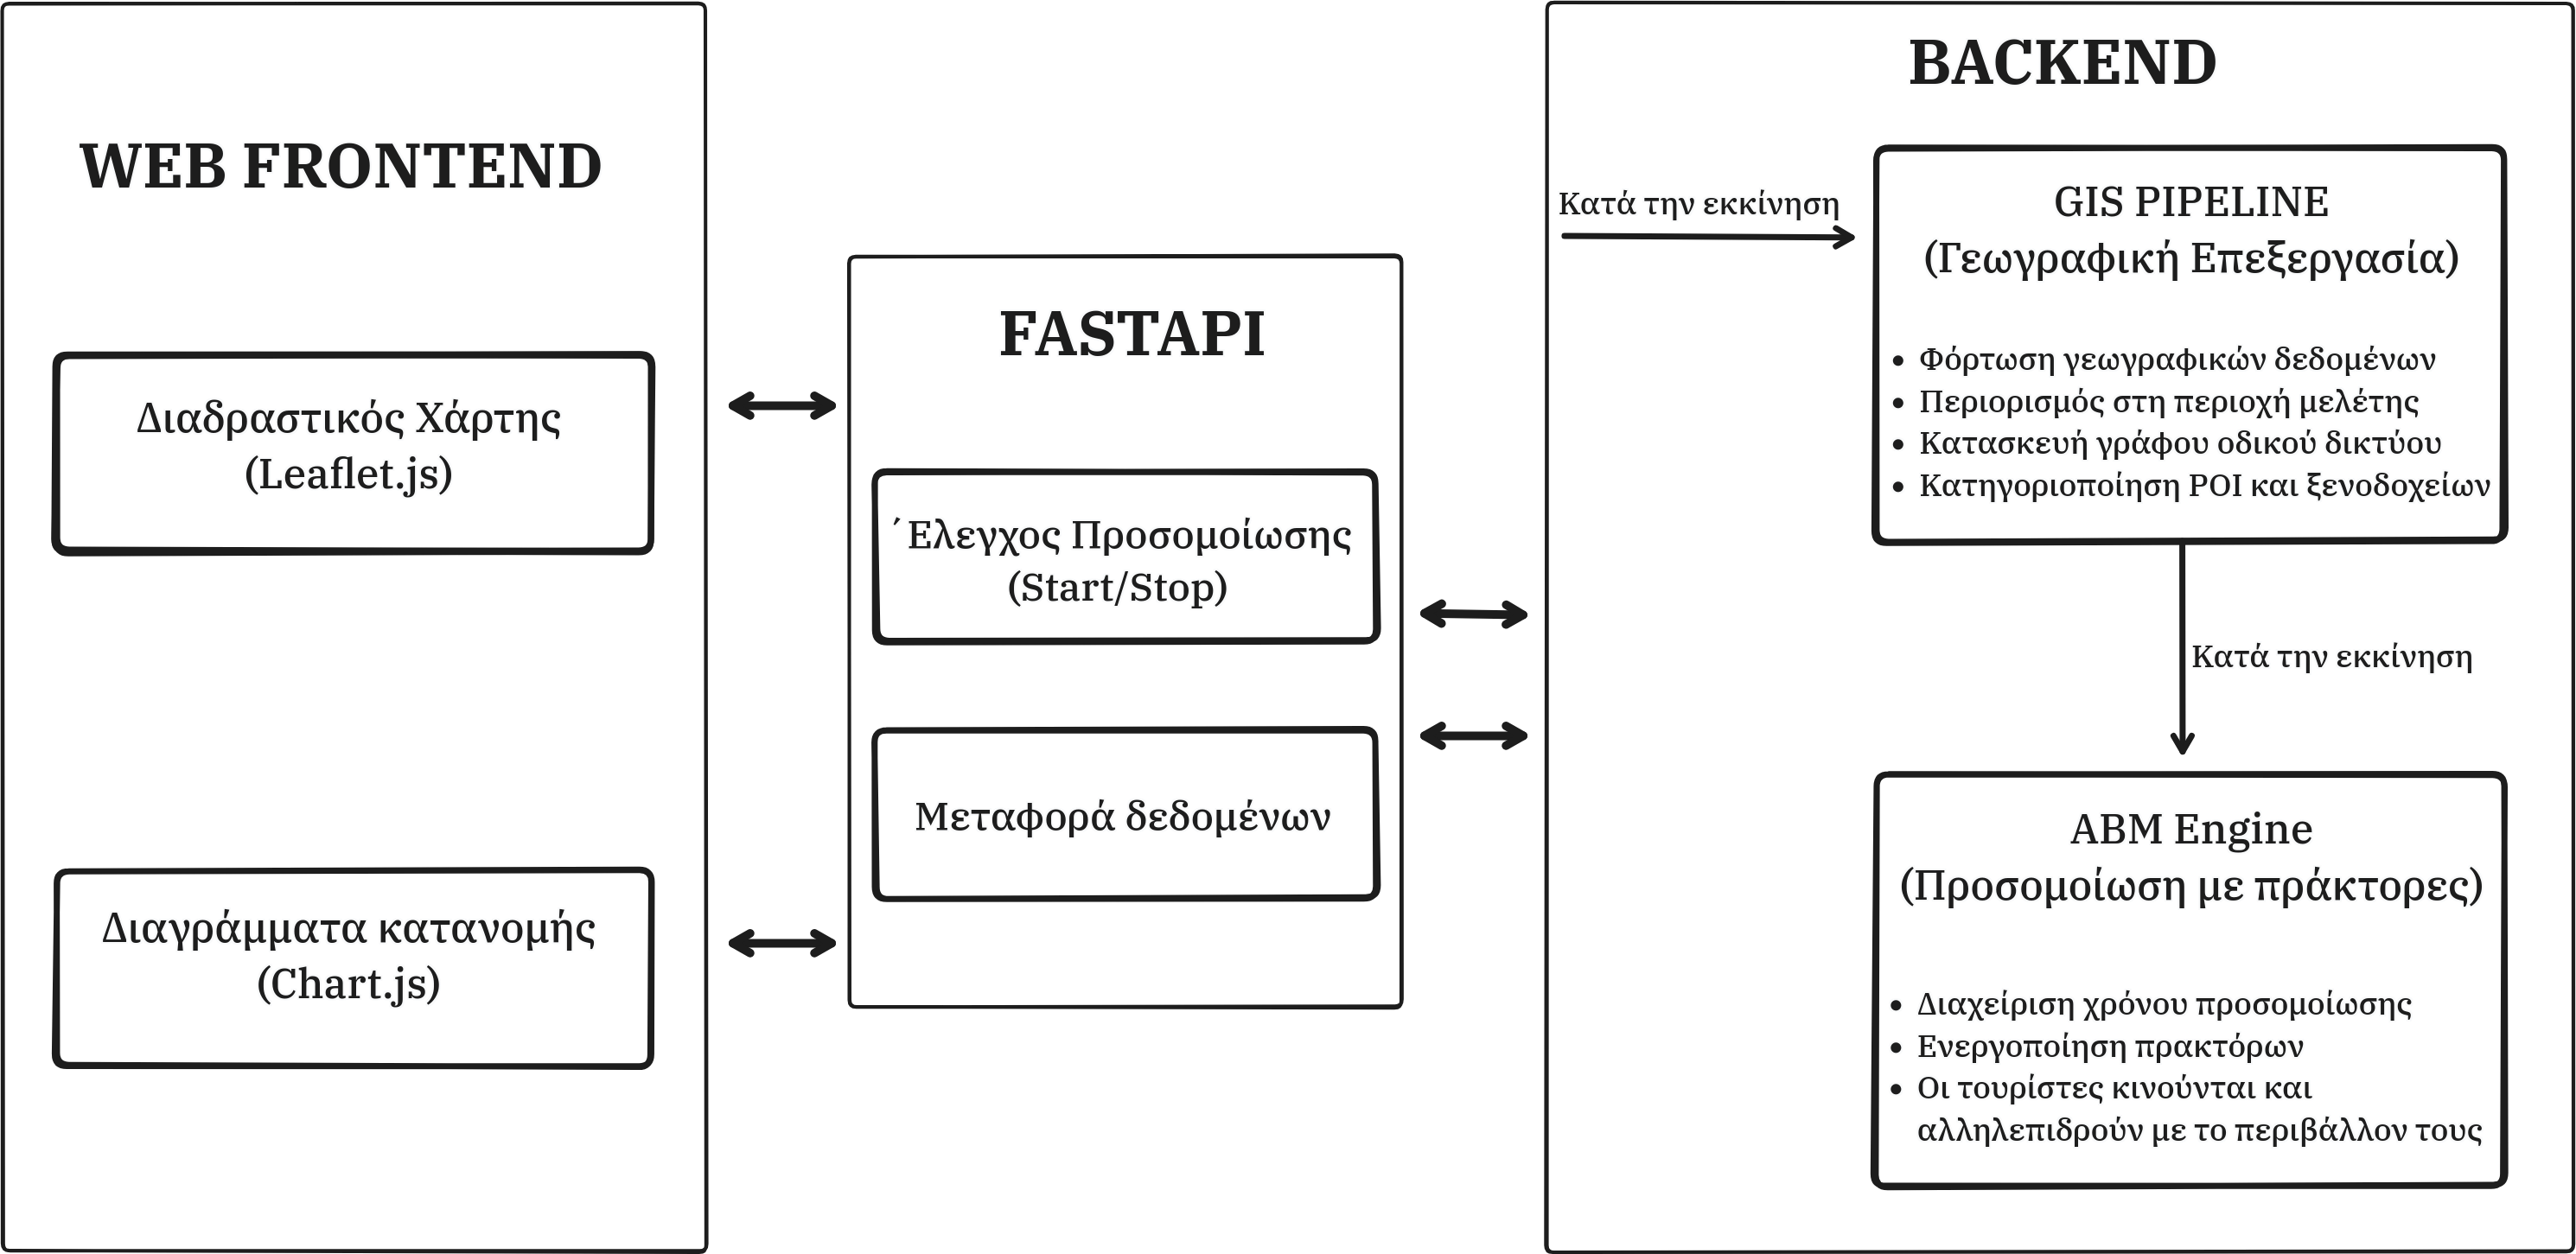
\includegraphics[width=\textwidth]{static/figures/system_architecture.png}
\caption{Αρχιτεκτονική Συστήματος}\label{system_architecture}
\end{figure}

\section{Σχεδιασμός Οδικού Δικτύου ως Γράφος}

Το οδικό δίκτυο αποτελεί τον χώρο κίνησης των πρακτόρων. Η
βασική σχεδιαστική απόφαση είναι η αναπαράστασή του ως μη
κατευθυνόμενος γράφος, όπου κάθε κόμβος αντιστοιχεί σε σημείο
διασταύρωσης ή άκρο δρόμου, και κάθε ακμή αντιστοιχεί σε τμήμα
δρόμου με γνωστή γεωμετρία. Αυτή η αναπαράσταση, όπως αναλύθηκε
στην Ενότητα 2.4, επιτρέπει την εφαρμογή αλγορίθμων πλοήγησης
και την ακριβή παρεμβολή θέσης πάνω στις ακμές.

Από το σύνολο των οδών που περιέχουν τα δεδομένα \en{OSM},
επιλέγονται μόνο εκείνες που επιτρέπουν πεζή κυκλοφορία,
αποκλείοντας ταχείες οδούς και αυτοκινητόδρομους που δεν είναι
προσβάσιμοι στους πεζούς. Η επιλογή αυτή εξασφαλίζει ότι η
κίνηση των πρακτόρων αντικατοπτρίζει ρεαλιστικά τη συμπεριφορά
των πεζών σε αστικό περιβάλλον.

Κάθε ακμή του γράφου αποκτά ένα βαθμολόγιο ελκυστικότητας που
συνδυάζει δύο παράγοντες: τον τύπο του δρόμου και την παρουσία
\en{POI} στην άμεση γειτονιά του. Αυτό το βαθμολόγιο
αντικατοπτρίζει την τάση των τουριστών να προτιμούν δρόμους με
εμπορική ή πολιτιστική δραστηριότητα, και αξιοποιείται από τον
αλγόριθμο πλοήγησης που περιγράφεται στην Ενότητα 4.4.2.

\section{Σχεδιασμός Πρακτόρων}

Το σύστημα περιλαμβάνει δύο διακριτούς τύπους πρακτόρων με
διαφορετική συμπεριφορά και ρόλο στην προσομοίωση. Και οι δύο
τύποι ζουν στον κοινό χώρο του μοντέλου, αλλά ο βαθμός
πολυπλοκότητάς τους διαφέρει σημαντικά.

\subsection{Μόνιμος Κάτοικος}

Ο μόνιμος κάτοικος \en{(resident)} αντιπροσωπεύει τον μόνιμο
πληθυσμό της πόλης. Είναι στατικός πράκτορας, δηλαδή δεν
κινείται κατά τη διάρκεια της προσομοίωσης, και ο ρόλος του
είναι να αποτυπώνει τον αντίκτυπο του τουρισμού στην ποιότητα
ζωής των κατοίκων μέσω μεταβλητής ευτυχίας.

Η ευτυχία \en{(happiness)} μεταβάλλεται ανάλογα με τον αριθμό
τουριστών που βρίσκονται στην άμεση γειτονιά του κατοίκου:
αυξάνεται όταν δεν υπάρχουν τουρίστες κοντά, μειώνεται
σταδιακά με την αύξηση του συνωστισμού και επαναφέρεται στην
αρχική τιμή στην αρχή κάθε νέας ημέρας. Η απλότητα αυτού του
μοντέλου είναι συνειδητή. Ο κάτοικος λειτουργεί ως
$``$αισθητήρας$"$ τουριστικής πίεσης στον χώρο, όχι ως
αυτόνομος πράκτορας με δικές του πρωτοβουλίες.

\subsection{Τουρίστας}

Ο τουρίστας \en{(tourist)} είναι ο πολυπλοκότερος πράκτορας
του συστήματος. Κινείται πάνω στο οδικό δίκτυο και εμφανίζει
σύνθετη ημερήσια συμπεριφορά που περιλαμβάνει φάσεις ύπνου,
ενεργή περιήγηση και επίσκεψη \en{POI}. Κάθε τουρίστας φέρει
χαρακτηριστικά περιβαλλοντικής επίδρασης (θόρυβος, ρύπανση)
και παρακολουθεί την ικανοποίησή του ανάλογα με τις συνθήκες
συνωστισμού που συναντά.

Ο τουρίστας όταν ανακαλύπτει ένα νέο σημείο ενδιαφέροντος,
κατευθύνεται προς αυτό και το επισκέπτεται. Διαθέτει ωστόσο
δυνατότητα παρεκτροπής. Για παράδειγμα, μπορεί να κάνει στάση
για καφέ καθώς κατευθύνεται προς ένα μουσείο. Σε αυτή την
περίπτωση, το καφέ γίνεται πρωτεύον στόχος του τουρίστα, ενώ
το μουσείο από πρωτεύον γίνεται δευτερεύον στόχος. Η απόφαση
παρεκτροπής είναι στοχαστική και εξαρτάται από το \en{tier}
του \en{POI}. Κανένας τουρίστας δεν επισκέπτεται δύο φορές
το ίδιο \en{POI}.

Η πλοήγηση στο οδικό δίκτυο βασίζεται σε υβριδικό αλγόριθμο
που συνδυάζει δύο κριτήρια: την ευθυγράμμιση με την κατεύθυνση
προς τον στόχο και την ελκυστικότητα της ακμής. Η στάθμιση
μεταξύ των δύο κριτηρίων προσαρμόζεται δυναμικά ανάλογα με
την απόσταση από τον στόχο, ώστε ο τουρίστας να διατηρεί
την κατεύθυνσή του όταν ο στόχος είναι μακριά, ενώ να
εξερευνά πιο ελεύθερα όταν βρίσκεται κοντά.

\subsection{Σύστημα Ιεραρχίας \en{POI}}

Τα Σημεία Ενδιαφέροντος κατηγοριοποιούνται σε τρία επίπεδα
βάσει της τουριστικής τους σημασίας και του τύπου εμπειρίας
που προσφέρουν. Η ιεράρχηση αυτή αντικατοπτρίζει την πραγματική
συμπεριφορά των τουριστών, οι οποίοι οργανώνουν την ημέρα τους
γύρω από λίγα κεντρικά αξιοθέατα και συμπληρώνουν την εμπειρία
τους με επισκέψεις σε εστιατόρια και καταστήματα.

Το \en{Tier A} περιλαμβάνει τα σημεία υψηλής τουριστικής αξίας,
όπως μουσεία, αξιοθέατα, μνημεία, αρχαιολογικούς χώρους και
παρόμοιους προορισμούς. Αποτελεί τον κύριο λόγο επίσκεψης μιας
πόλης. Το \en{Tier B} περιλαμβάνει καταστήματα εστίασης και
αναψυχής, που λειτουργούν ως δευτερεύοντες προορισμοί που
εμπλουτίζουν την εμπειρία της περιήγησης. Το \en{Tier C}
περιλαμβάνει καταστήματα λιανικής, που αποτελούν τριτεύοντες
προορισμούς ευκαιριακής επίσκεψης.

Ο αλγόριθμος επιλογής στόχου ακολουθεί αυστηρή ιεραρχία:
ο τουρίστας αναζητά πάντα πρώτα \en{POI Tier A}, και μόνο αν
δεν εντοπίσει κανένα στρέφεται σε κατώτερα \en{tiers}. Αυτή
η ιεραρχία εφαρμόζεται τόσο κατά την έναρξη της ημέρας όσο
και κατά την ελεύθερη περιπλάνηση. Η διάρκεια επίσκεψης
διαφέρει ανά \en{tier}, αντικατοπτρίζοντας τον διαφορετικό
χαρακτήρα κάθε κατηγορίας \en{POI}.

\section{Ξενοδοχεία και Ανάθεση Πρακτόρων}

Τα ξενοδοχεία αποτελούν τη βάση επιστροφής των τουριστών κατά
τις ώρες ύπνου και αντλούνται αυτόματα από τα δεδομένα \en{OSM}.
Σε περίπτωση που η βάση δεδομένων δεν περιέχει επαρκή αριθμό
ξενοδοχείων για την επιλεγμένη πόλη, το σύστημα χρησιμοποιεί
εναλλακτικά \en{POI} υψηλής επισκεψιμότητας ως σημεία αναφοράς,
εξασφαλίζοντας τη λειτουργία του μοντέλου ανεξαρτήτως της
πληρότητας των δεδομένων.

Κατά τη δημιουργία κάθε τουρίστα, το σύστημα του αναθέτει
αυτόματα ένα ξενοδοχείο μέσω αλγορίθμου ισορροπημένης κατανομής,
ο οποίος αποφεύγει την υπερφόρτωση συγκεκριμένων ξενοδοχείων.
Η ανάθεση παραμένει σταθερή για όλη τη διάρκεια της προσομοίωσης.

Η μετάβαση στη φάση ύπνου αντιμετωπίζεται με απλοποίηση.
Ο τουρίστας μεταφέρεται άμεσα στη θέση του ξενοδοχείου του,
αντί να πλοηγηθεί εκεί μέσω του οδικού δικτύου. Αυτή η
σχεδιαστική επιλογή είναι συνειδητή. Αποφεύγει πολυπλοκότητα
που δεν προσθέτει ερευνητική αξία, εφόσον το ενδιαφέρον της
προσομοίωσης εστιάζεται στη δραστηριότητα κατά τις ώρες εγρήγορσης.